\chapter{Conclusion and Outlook}
\label{Con}
\section{Conclusion}
\label{Con:Con}

During this master thesis the Routing Protocol for LLNs (RPL) has been studied. The study was based on the simulation of BLIP 2.0 with the rfxlink radio stack using the simulation tool \texttt{TOSSIM}.

Low power consumption and low control message overhead are crucial due to the resource constraints in LLNs. In RPL, three kinds of control messages are defined - DIS and DIO messages are sent to construct and maintain upward routes while DAOs are used to discover and maintain downward routes. The node which is closer to the root tends to send more control messages than the further ones. Furthermore, RPL uses the Trickle algorithm to control the generation of DIOs. In various scenarios, it efficiently reduces the control message overhead as soon as the routing topology is stabilized. For the root which only sends DIOs, the typical mean number of control messages it sends during the first 10 minutes is 11 and 2.5 during the second 10 minutes. For non-root node, the control message decreasing rate usually varies between half to a quarter.

As soon as the nodes boot up, DIOs are sent to help nodes discovering the default routes. The sending of DIO messages is governed by the Trickle timer. Due to the Trickle algorithm, the default route discovery times of the single hop nodes are uniform distributed. For a multi-hop node, the distribution of the default route discovery time is the summation of multiple uniform distributions, thus resulting an normal distribution. By adding the default route discovery time distributions of all the nodes in a network, one can get a CDF of the whole network which shows almost a uniform increase again.

Objective Functions (OFs) are defined for RPL to meet different optimization requirements. OF0 and MRHOF are two OFs which are implemented in BLIP 2.0. The performances are evaluated in terms of RTT and packet loss with the application \texttt{UDPEcho}. The simulation results show that OF0 has a equally good performance as MRHOF in simple and low density scenarios. For more dense scenarios, OF0 has unstable performances due to the fact that it chooses routes without using link layer information. On the other hand, MRHOF with ETX routing metric has not only less packet loss and lower RTT than OF0 in larger and more complicated topologies, but also a more stable performance.

During the course of simulation several bugs that were present in RPL/OFs and BLIP were fixed and have been applied to the upstream repository.

\section{Outlook}
\label{outlook}

% mab: please let the outlook be checked by some other student for
% spelling errors, grammar and content.

% e.g. I don't understand the following sentence:
%, there are far more that routing-related issues facing the LLNs.

% Would you split the outlook items into: scenario, metrics, protocols, etc.

In the future the complexity of the simulated system can be improved. Whereas only a handful of parameters were studied in this thesis, there are far more routing-related issues facing the LLNs.
 
First of all, more scenarios can be created to further exam the performance of RPL. An example would be the scenario of uneven internode spacing - what will the performance of RPL be if the neighboring node spacing is not as regular as the the scenarios created in this thesis. Non-equidistant node spacing needs to be included into future simulations. Another improvement that can be made is to simulate with the real-world noise trace and path attenuation which will increase the fidelity of the simulation. 

Addition to scenario, more metrics can be used to evaluate the performance of RPL. RPL employs two DODAG repair mechanisms - gloable repair which will increase the DODAG version number and local repair which repairs  a local DODAG within the DODAG version number. Link failures can be added to the simulation to exam the behavior of both repair mechanisms.

In this thesis, simulation with the application \texttt{UDPEcho} shows the basic performances of RPL, but there are many other applications which are worth exploring. Currently, a client and server implementation of the Constrained Application Protocol(CoAP) have been done for TinyOS/BLIP 2.0 in~\cite{TP11} and the simulation of the line scenario and the grid scenario has been presented. In the future, some real-life scenario with CoAP can be simulated for evaluation. One practical real-life scenario would be the "Intelligent Container" project at the University of Bremen. Figure~\ref{fig:container} shows an example cargo container scenario with 32 child nodes and 1 border router. This scenario defines five types of connections depending on the position of the sensor nodes:

\begin{figure}[htbp]
  \begin{center}
    \leavevmode
      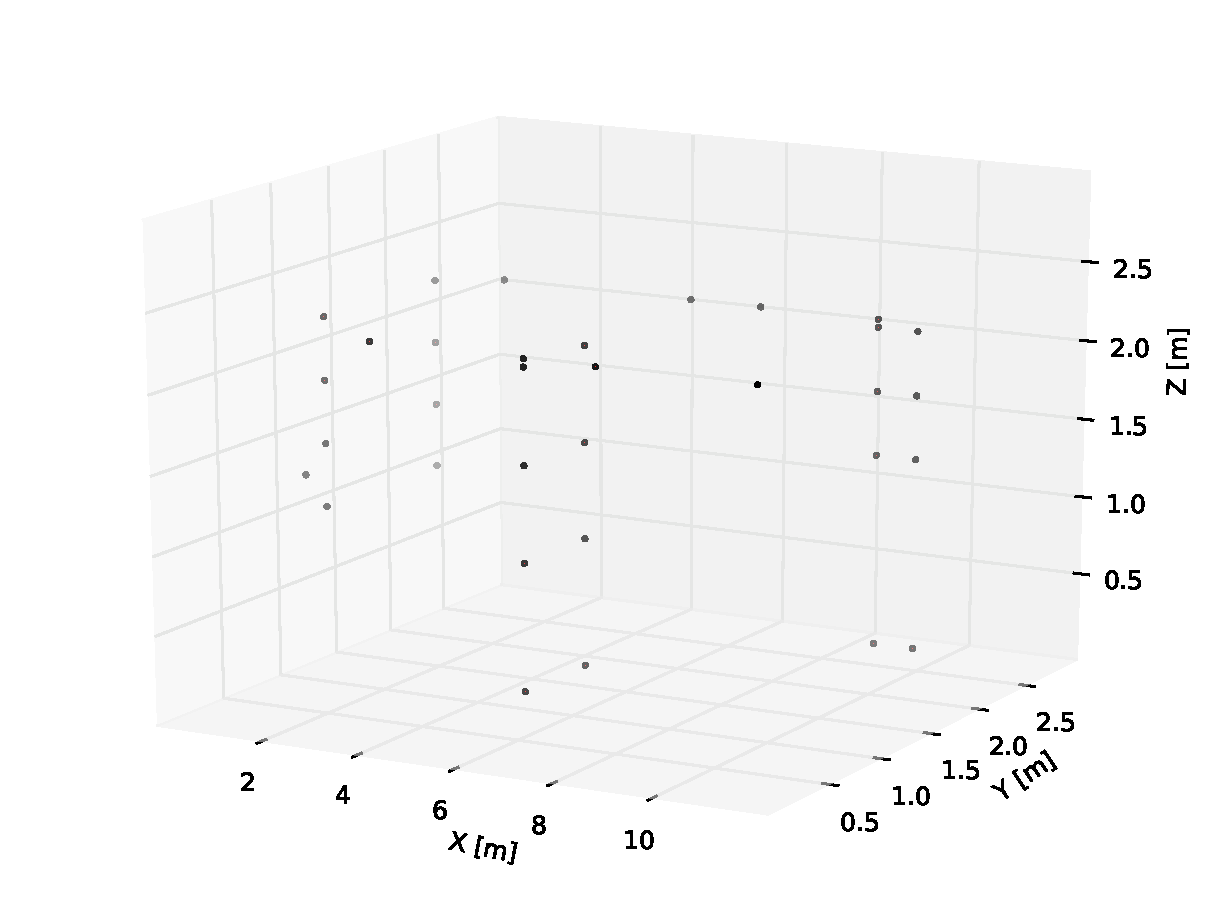
\includegraphics[scale=0.45]
      {Pics/container.pdf}
   \caption{A cargo container scenario with 32 sensor nodes and 1 border router}
    \label{fig:container}
  \end{center}
\end{figure}

\begin{itemize}
\item Connections between nodes on the roof of the container.
\item Connections between nodes on the roof of the container and those on top of the pallets.
\item Connections between nodes on the top of the pallets.
\item Connections between nodes on top of the pallets and inside the goods.
\item Connections between nodes that are inside the goods.
\end{itemize}

The performance of CoAP on top of BLIP 2.0 under this real-life container scenario can be evaluated from the simulation results.


